% Template for PLoS
% Version 3.1 February 2015
%
% To compile to pdf, run:
% latex plos.template
% bibtex plos.template
% latex plos.template
% latex plos.template
% dvipdf plos.template
%
% % % % % % % % % % % % % % % % % % % % % %
%
% -- IMPORTANT NOTE
%
% This template contains comments intended 
% to minimize problems and delays during our production 
% process. Please follow the template instructions
% whenever possible.
%
% % % % % % % % % % % % % % % % % % % % % % % 
%
% Once your paper is accepted for publication, 
% PLEASE REMOVE ALL TRACKED CHANGES in this file and leave only
% the final text of your manuscript.
%
% There are no restrictions on package use within the LaTeX files except that 
% no packages listed in the template may be deleted.
%
% Please do not include colors or graphics in the text.
%
% Please do not create a heading level below \subsection. For 3rd level headings, use \paragraph{}.
%
% % % % % % % % % % % % % % % % % % % % % % %
%
% -- FIGURES AND TABLES
%
% Please include tables/figure captions directly after the paragraph where they are first cited in the text.
%
% DO NOT INCLUDE GRAPHICS IN YOUR MANUSCRIPT
% - Figures should be uploaded separately from your manuscript file. 
% - Figures generated using LaTeX should be extracted and removed from the PDF before submission. 
% - Figures containing multiple panels/subfigures must be combined into one image file before submission.
% For figure citations, please use "Fig." instead of "Figure".
% See http://www.plosone.org/static/figureGuidelines for PLOS figure guidelines.
%
% Tables should be cell-based and may not contain:
% - tabs/spacing/line breaks within cells to alter layout or alignment
% - vertically-merged cells (no tabular environments within tabular environments, do not use \multirow)
% - colors, shading, or graphic objects
% See http://www.plosone.org/static/figureGuidelines#tables for table guidelines.
%
% For tables that exceed the width of the text column, use the adjustwidth environment as illustrated in the example table in text below.
%
% % % % % % % % % % % % % % % % % % % % % % % %
%
% -- EQUATIONS, MATH SYMBOLS, SUBSCRIPTS, AND SUPERSCRIPTS
%
% IMPORTANT
% Below are a few tips to help format your equations and other special characters according to our specifications. For more tips to help reduce the possibility of formatting errors during conversion, please see our LaTeX guidelines at http://www.plosone.org/static/latexGuidelines
%
% Please be sure to include all portions of an equation in the math environment.
%
% Do not include text that is not math in the math environment. For example, CO2 will be CO\textsubscript{2}.
%
% Please add line breaks to long display equations when possible in order to fit size of the column. 
%
% For inline equations, please do not include punctuation (commas, etc) within the math environment unless this is part of the equation.
%
% % % % % % % % % % % % % % % % % % % % % % % % 
%
% Please contact latex@plos.org with any questions.
%
% % % % % % % % % % % % % % % % % % % % % % % %

\documentclass[10pt,letterpaper]{article}
\usepackage[top=0.85in,left=2.75in,footskip=0.75in]{geometry}

% Use adjustwidth environment to exceed column width (see example table in text)
\usepackage{changepage}

% Use Unicode characters when possible
\usepackage[utf8]{inputenc}

% textcomp package and marvosym package for additional characters
\usepackage{textcomp,marvosym}

% fixltx2e package for \textsubscript
\usepackage{fixltx2e}

% listings package for code
\usepackage{listings}

% amsmath and amssymb packages, useful for mathematical formulas and symbols
\usepackage{amsmath,amssymb}

% cite package, to clean up citations in the main text. Do not remove.
\usepackage{cite}

% Use nameref to cite supporting information files (see Supporting Information section for more info)
\usepackage{nameref,hyperref}

% line numbers
\usepackage[right]{lineno}

% ligatures disabled
\usepackage{microtype}
\DisableLigatures[f]{encoding = *, family = * }

% rotating package for sideways tables
\usepackage{rotating}

% Remove comment for double spacing
%\usepackage{setspace} 
%\doublespacing

% Text layout
\raggedright
\setlength{\parindent}{0.5cm}
\textwidth 5.25in 
\textheight 8.75in
\setlength{\headheight}{28pt} 

% Bold the 'Figure #' in the caption and separate it from the title/caption with a period
% Captions will be left justified
\usepackage[aboveskip=1pt,labelfont=bf,labelsep=period,justification=raggedright,singlelinecheck=off]{caption}

% Use the PLoS provided BiBTeX style
\bibliographystyle{plos2015}

% Remove brackets from numbering in List of References
\makeatletter
\renewcommand{\@biblabel}[1]{\quad#1.}
\makeatother

% Leave date blank
\date{}

% Header and Footer with logo
\usepackage{lastpage,fancyhdr,graphicx}
\usepackage{epstopdf}
\pagestyle{myheadings}
\pagestyle{fancy}
\fancyhf{}
\lhead{
\includegraphics[width=2.0in]{/Users/dphamnyghonca/Desktop/gloor/msc_thesis_2016/unifrac_paper/PLOS-submission.eps}}
\rfoot{\thepage/\pageref{LastPage}}
\renewcommand{\footrule}{\hrule height 2pt \vspace{2mm}}
\fancyheadoffset[L]{2.25in}
\fancyfootoffset[L]{2.25in}
\lfoot{\sf PLOS}

%% Include all macros below

\newcommand{\lorem}{{\bf LOREM}}
\newcommand{\ipsum}{{\bf IPSUM}}

%% END MACROS SECTION


\begin{document}
\vspace*{0.35in}

% Title must be 250 characters or less.
% Please capitalize all terms in the title except conjunctions, prepositions, and articles.
\begin{flushleft}
{\Large
\textbf\newline{Expanding the UniFrac toolbox}
}
\newline
% Insert author names, affiliations and corresponding author email (do not include titles, positions, or degrees).
\\
Ruth G Wong\textsuperscript{1 \Yinyang},
Jia R Wu\textsuperscript{1 \Yinyang},
Gregory B Gloor\textsuperscript{1 *}
\\
\bigskip
\bf{1} Department of Biochemistry, University of Western Ontario, London, Ontario, Canada
\\
\bigskip

% Insert additional author notes using the symbols described below. Insert symbol callouts after author names as necessary.
% 
% Remove or comment out the author notes below if they aren't used.
%
% Primary Equal Contribution Note
\Yinyang These authors contributed equally to this work.

% Additional Equal Contribution Note
% Also use this double-dagger symbol for special authorship notes, such as senior authorship.
% \ddag These authors also contributed equally to this work.

% Current address notes
%\textcurrency a Insert current address of first author with an address update
% \textcurrency b Insert current address of second author with an address update
% \textcurrency c Insert current address of third author with an address update

% Deceased author note
%\dag Deceased

% Group/Consortium Author Note
%\textpilcrow Membership list can be found in the Acknowledgments section.

% Use the asterisk to denote corresponding authorship and provide email address in note below.
* ggloor@uwo.ca

\end{flushleft}
% Please keep the abstract below 300 words
\section*{Abstract}
Microbiome analysis is frequently performed using the UniFrac distance metric to separate groups. Here we demonstrate that unweighted UniFrac is highly sensitive to rarefaction instance and to sequencing depth in uniform data sets. We show that this arises because of subcompositional effects. We introduce information UniFrac and centered ratio UniFrac, two new weightings that are not sensitive to rarefaction and allow greater separation of outliers than classic unweighted and weighted UniFrac. With this expansion of the UniFrac toolbox, we hope to empower researchers to extract more varied information from their data.

% Please keep the Author Summary between 150 and 200 words
% Use first person. PLOS ONE authors please skip this step. 
% Author Summary not valid for PLOS ONE submissions.   
% \section*{Author Summary}
% Lorem ipsum dolor sit amet, consectetur adipiscing elit. Curabitur eget porta erat. Morbi consectetur est vel gravida pretium. Suspendisse ut dui eu ante cursus gravida non sed sem. Nullam sapien tellus, commodo id velit id, eleifend volutpat quam. Phasellus mauris velit, dapibus finibus elementum vel, pulvinar non tellus. Nunc pellentesque pretium diam, quis maximus dolor faucibus id. Nunc convallis sodales ante, ut ullamcorper est egestas vitae. Nam sit amet enim ultrices, ultrices elit pulvinar, volutpat risus.

\linenumbers

\section*{Introduction}
In 2005, Lozupone et al introduced the UniFrac distance metric, a measure to calculate the difference between microbiomes that incorporated phylogenetic distance \cite{lozupone2005unifrac}. The goal of UniFrac was to enable objective comparison between microbiome samples from different conditions. In 2007, Lozupone added a proportional weighting to the original unweighted method \cite{lozupone2007quantitative}. Since then, papers reporting these metrics have garnered over a thousand citations, and enabled research about everything from how kwashiorkor causes malnutrition \cite{smith2013gut} to how people can have similar microbiomes to their pet dogs \cite{song2013cohabiting}. Except for generalized UniFrac, used to make hybrid unweighted and weighted UniFrac comparisons \cite{chen2012associating}, few advances in the metric have occurred since 2007. In this paper we examine a data set where unweighted UniFrac gives misleading results, and discuss some alternative weightings for UniFrac.

\subsection{Data}
UniFrac requires two pieces of data: A phylogenetic tree and a table of counts per inferred taxa per sample. This data is derived from a gene tag experiment, the most common of which is the 16S rRNA gene tag experiment for microbiome research [CITE]. A gene tag experiment is run by amplifying the gene tag through PCR, and then sequencing the resulting amplicon.

\paragraph{Operational Taxonomic Units}\mbox{}\\
Unlike more distinct species, such as mammalian species, bacterial species are not well defined. Bacterial genomes are highly variable, and regions used to identify bacteria vary in a continuum rather than clusters of similar sequences.

Historically bacteria that are have 97\% identity in a variable region are considered to be the same taxa. The 97\% cutoff was arbitrarily chosen to best map sequence data to bacterial classifications. This threshold maximizes the grouping of bacteria classified as the same species while minimizing the grouping of bacteria classified as different species. Before sequencing bacterial classification was often done by appearance or by metabolic products, so there are outliers where bacteria classified in the same species are actually genetically very different, or bacteria classified in different genus are genetically very similar.

However, it is difficult to determine how a batch of sequences should be partitioned into groups of 97\% identity. One way is to perform a clustering algorithm (using software such as UCLUST \cite{edgar2010search}) that optimally partitions the groups and then later assign taxonomic identity by matching the sequences with public databases, such as SILVA \cite{quast2013silva}, the Ribosomal Database Project \cite{cole2009ribosomal}, and Greengenes \cite{desantis2006greengenes}. Another way is to start off with seed sequences from known bacteria and perform the clustering such that the 97\% identity groups are centered on the seed sequences. In any case, the resulting taxonomic groupings are known as Operational Taxonomic Units (OTUs), and are used consistently within the same experiment. While OTUs can be annotated with standard taxonomic names such that results can be compared between experiments, technically the taxonomic groupings used by different experiments are not the same.

Grouping of amplicon sequences into OTUs allows for the data to be summarized into a table of counts per OTU per sample.

\paragraph{Phylogenetic tree}\mbox{}\\
To generate the phylogenetic tree \cite{ciccarelli2006toward}, a representative sequence is taken from each of the cluster of sequences that belong to each OTU. If seed sequences were used to generate the OTU, then these can be used for the phylogenetic tree, otherwise a sequence in the center of the cluster should be selected.

The phylogenetic tree is created through a multiple sequence alignment with the representative OTU sequences, using software such as MUSCLE \cite{edgar2004muscle}. Each leaf of the tree represents one of the OTUs, and each of the branches of the tree has a length. Additionally, the tree needs to be rooted for the UniFrac calculation to be performed. This can be done by rooting the tree by its midpoint, which can be performed by software such as the phangorn R package \cite{schliep2011phangorn}.

\subsection{Unweighted UniFrac}
Unweighted UniFrac \cite{lozupone2005unifrac} uses an inferred evolutionary distance to measure similarity between samples. It requires a reference phylogenetic tree containing all the taxa present in the samples to be examined, plus information about which taxa were detected in each sample. The calculation is performed by dividing the branch lengths shared between the two samples by the branch lengths covered by either sample. A distance of 0 means that the samples are identical, and a distance of 1 means that the two samples share no taxa in common.

\begin{figure}[h]
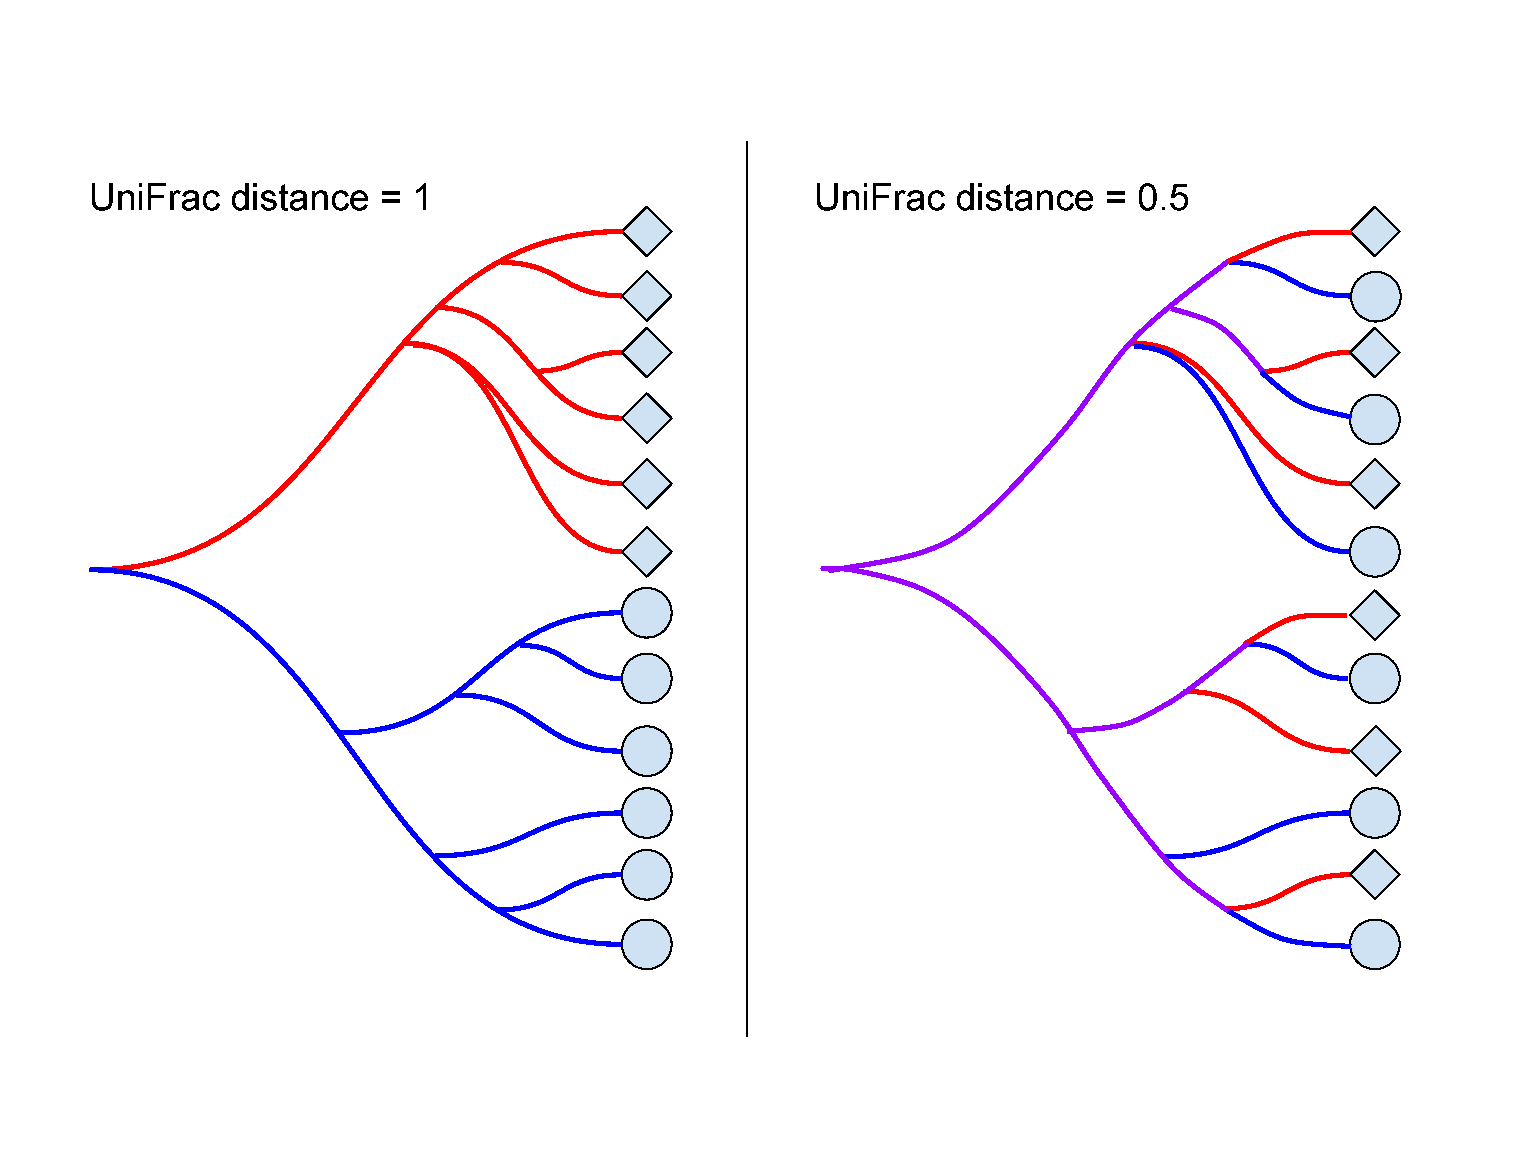
\includegraphics[scale=0.5]{/Users/dphamnyghonca/Desktop/gloor/msc_thesis_2016/unifrac_paper/unifrac_distance.eps}
\caption{{\bf Unweighted UniFrac.}
When two samples do not share any branches of the phylogenetic tree, the unweighted UniFrac distance is maximized at 1. When two samples share half of their branch lengths on the phylogenetic tree, the unweighted UniFrac distance is 0.5. If the two samples contain exactly the same taxa, the unweighted UniFrac distance is minimized at 0, since the samples share all branches.}
\label{fig1}
\end{figure}

\subsection{Weighted UniFrac}
Weighted UniFrac \cite{lozupone2007quantitative} is an implementation of the Kantorovich–Rubinstein distance in mathematics, also known as the earth mover’s distance \cite{evans2012phylogenetic}. Rather than looking only at the presence or absence of taxa, each branch length of the phylogenetic tree is weighted by the difference in proportional abundance of the taxa between the two samples.

This technique reduces the problem of low abundance taxa being represented as a 0 or by a low count depending on sampling depth. In unweighted UniFrac, such taxa would flip from absent to present, and could skew the measurement: this would be especially problematic if the taxa are on a long branch. In weighted UniFrac, low abundance taxa have a much lower weight and so will have a lower impact on the total distance reported by the metric.

UniFrac is constituted as either a presence/absence (unweighted UniFrac) \cite{lozupone2005unifrac}, a linear proportion (weighted UniFrac) \cite{lozupone2007quantitative}, or some combination of the two (generalized UniFrac) \cite{chen2012associating}. However, the data are not linear, because the sum of the total number of reads is constrained by the sequencing machinery \cite{friedman2012inferring} \cite{fernandes2013anova} \cite{fernandes2014unifying} \cite{lovell2015proportionality}. Alternative weightings and non-linear transformations of data need to be explored. Furthermore, unweighted UniFrac is known to be unreliable, but it is not generally known or understood how this can impact results.

% You may title this section "Methods" or "Models". 
% "Models" is not a valid title for PLoS ONE authors. However, PLoS ONE
% authors may use "Analysis" 
\section*{Materials and Methods}

\subsection{Analytical techniques}

\paragraph{Rarefaction}\mbox{}\\
Rarefaction normalizes the samples OTU counts to a standard sequencing depth \cite{simberloff1978use}. This resulting table can be thought of as a random point estimate of the dataset, as the output is a sub-sample of the original table. This standardization process is recommended by the authors of UniFrac \cite{de2011evaluation} in order to account for the sensitivity of UniFrac to sequencing depth.

Rarefactions can be performed using the Qiime software \cite{caporaso2010qiime} or using the vegan package in R \cite{oksanen2007vegan}.

\paragraph{Unweighted UniFrac}\mbox{}\\
Unweighted UniFrac is calculated based on the presence or absence of counts for each branch in the phylogenetic tree, when comparing two samples. A branch belongs to a sample when at least one of the OTUs in the leaves below it have a non-zero abundance. The formula for unweighted UniFrac is as follows, where $b$ is the set of branch lengths in the phylogenetic tree, and $A$ and $B$ represent the two samples being compared:

\begin{align*}
Unweighted_{AB} = \frac{\sum_{}{} b_{A} \triangle b_{B}}{\sum_{}{} b_{A} \cup b_{B}}
\end{align*}

The sum of the branch lengths that belong to one sample but not the other is divided by the sum of the branch lengths that belong to one or both samples.

\paragraph{Weighted UniFrac}\mbox{}\\
Weighted UniFrac \cite{lozupone2007quantitative} also incorporates each branch length of the phylogenetic tree, and weights them according to proportional abundance of the two samples. The formula for weighed UniFrac is as follows, where $A$ and $B$ are the two samples, $b$ is the set of branch lengths, and $\frac{A_{i}}{A_{T}}$ and $\frac{B_{i}}{B_{T}}$ are the proportional abundances associated with branch length $b_{i}$:

\begin{align*}
Weighted_{AB} = \sum_{i}^{n} b_{i} \times \left| \frac{A_{i}}{A_{T}} - \frac{B_{i}}{B_{T}} \right|
\end{align*}

\paragraph{Information UniFrac}\mbox{}\\
Information UniFrac is calculated by weighing each branch length by the difference in the uncertainty of the taxa abundance between the two samples. Uncertainty is calculated as follows, where p is the proportional abundance \cite{shannon2001mathematical}:

\begin{equation}\label{eq:schemeP} 
uncertainty = - p  \times log_{2}(p)
\end{equation}

If a sample is 50\% taxa A and 50\% taxa B, then the proportional abundances have maximum uncertainty about what taxa is likely to be seen in a given sequence read. If a sample is 80\% taxa A and 20\% taxa B, then there is less uncertainty, because a given sequence read is more likely to be taxa A. When the amount of uncertainty that a taxa has in one sample corresponds with the amount of uncertainty the same taxa has in a different sample, the abundance of that taxa is mutually informative between samples. Weighting UniFrac by uncertainty combines the the concept of uncertainty with phylogenetic relationships to identify taxa that are differentially informative between groups.

The formula for Information UniFrac is as follows:

\begin{align*}
Information_{AB} = \sum_{i}^{n} b_{i} \times \left| \frac{A_{i}}{A_{T}}log\left(\frac{A_{i}}{A_{T}}\right) - \frac{B_{i}}{B_{T}}log\left(\frac{B_{i}}{B_{T}}\right) \right|
\end{align*}

\paragraph{Centered Ratio UniFrac}\mbox{}\\
In complex microbiome communities, there are very many bacterial taxa with a low level of counts. Taking the geometric mean of the proportional abundances of taxa in a microbiome sample represents an unbiased baseline \cite{aitchison1982statistical}. Experiments generally do not have power to detect differences at abundances below the mean \cite{fernandes2013anova}. Centering the proportional abundances around the geometric mean thus allows one to examine the data in context, muting differences that are close to baseline and accentuating outliers. The formula for centered ratio UniFrac is as follows, where $gm$ is the geometric mean:

\begin{align*}
Centered Ratio_{AB} = \sum_{i}^{n} b_{i} \times \left| \frac{\frac{A_{i}}{A_{T}}}{gm(A_{i})} - \frac{\frac{B_{i}}{B_{T}}}{{gm(B_{i})}} \right|
\end{align*}

Note that the geometric mean is calculated by combining all children in the subtree of $b_{i}$ into $\frac{A_{i}}{A_{T}}$ for sample $A$ or $\frac{B_{i}}{B_{T}}$ for sample $B$, and including the rest of the single taxa proportional abundances separately. The one combined proportional abundance and the remaining single taxa proportional abundances are input into the geometric mean formula, as set $a$:

\begin{align*}
gm(a) = \left( \prod_{i}^{n} a_{i}\right)^{1/n}
\end{align*}

One challenge when it comes to the analysis of read count data is the presence of zero counts. Whether a low-abundance taxa appears in the data as a zero or a low positive count is up to chance, and assuming that a zero count represents the absence of a taxa can be very misleading \cite{fernandes2013anova}. A Bayesian approach can be used to estimate the likelihood that a zero could be changed to a positive count if the sample were resequenced, implemented by the cmultRepl command in the zCompositions package in R \cite{palarea2015zcompositions}.

The use of this weighting for UniFrac produces measurements that violate the triangle inequality, such that Euclidean statistics are technically invalid. Thus this, like the Bray-Curtis metric, is a dissimilarity, not a distance.

For this paper, we calculate UniFrac metrics using a custom R script, which includes unweighted UniFrac, weighted UniFrac, information UniFrac, and centered ratio UniFrac: https://github.com/ruthgrace/exponentUnifrac/blob/master/UniFrac.r

\paragraph{Bray-Curtis dissimilarity metric}\mbox{}\\
The Bray Curtis dissimilarity metric \cite{beals1984bray} quantifies how dissimilar two sites are based on counts. A index of 0 means that two samples are identical, while a index of 1 means samples do not share any species. It is computed as a proportion through the formula:

\begin{align*}
C_{ij} &= 1 - \frac{2C_{ij}}{S_{i} + S_{j}} \\
\text{where}~C_{ij}&= \text{dissimilarity index bound by [0,1]} \\
  S_{i} &= \text{Specimen counts at site i} \\
  S_{j} &= \text{Specimen counts at site j} \\
\end{align*}

\subsection{Data preparation}
The data used comes in the form of a table of counts per operational taxonomic unit per sample, plus a phylogenetic tree. All of our data are derived from 16S rRNA gene tag sequencing experiments.

\paragraph{Tongue dorsum data set}\mbox{}\\
The tongue dorsum data set is a collection of 60 microbiome samples taken from the tongues of healthy participants.

Samples from this experiment were sourced from the Human Microbiome Project \cite{turnbaugh2007human} Qiime Community profiling v35 otu tables (\url{http://hmpdacc.org/HMQCP/}).

Analysis of the data was conducted on a Late 2011 15 inch MacBook Pro 2.4 GHz i7 with 16GB of 1333 MHz DDR3 RAM. Rarefaction was conducted through Qiime version 1.8.0-20140103, and generation of the ellipse figures was done in R version 3.2.3 (2015-12-10) "Wooden Christmas-Tree" x86\_64-apple-darwin13.4.0 (64 bit).

A principal coordinate analysis is drawn from each distance matrix per metric, and for the first principal coordinate of each metric, Vres is computed per each first principal coordinate as defined by the formula:

\begin{align*}
  V_{res} &=\frac{|V_1 - V_i|}{range(V_1, V_i)} \\
  \text{where}~V_{res}&= \text{Set of computed PC1s,} \\
  V_1 &= \text{Reference PC1 (the first),} \\
  V_i &= \text{Each subsequent PC1,} \\
\end{align*}

\paragraph{Tongue dorsum and buccal mucosa data set}\mbox{}\\
The tongue dorsum and buccal mucosa data set is a collection of 30 microbiome samples taken from the tongues of healthy participants, plus 30 microbiome samples taken from the buccal mucosa (cheek) of a different set of healthy participants.

To create this data set, thirty random samples were selected from the tongue site of the Human Microbiome Project \cite{turnbaugh2007human} and thirty random samples from the buccal mucosa site. Samples were filtered so that only samples with 5000 to 10,000 reads were included.

Read counts from the HMP data set were rarefied to the smallest total read count per sample using the vegan R package \cite{oksanen2007vegan} before the unweighted UniFrac distance was calculated. Weighted, information, and centered log UniFrac were calculated on the data set without rarefaction. The resulting distances were plotted for principal coordinate analysis.

The script used to run this analysis can be referenced at \url{https://github.com/ruthgrace/exponentUnifrac/blob/master/tongue_cheek_script.r}.

\paragraph{Breast milk data set}\mbox{}\\
The breast milk data set is a collection of 58 microbiome samples taken from lactating Caucasian Canadian women. The breast milk data set used here has also been published in the Microbiome Journal \cite{urbaniak2016human}.

The count table was analyzed using our custom UniFrac script. Data was rarefied to the sample with the smallest number of read counts (3072) before the unweighted UniFrac distance matrix was calculated. Non-rarefied data was used for weighted, information, and centered ratio UniFrac. Data was plotted using a principal components or coordinate analysis as appropriate.

The script used to run this analysis can be referenced at \url{https://github.com/ruthgrace/exponentUnifrac/blob/master/breastmilk_script.r}.

% Results and Discussion can be combined.
\section*{Results}

\subsection{Unweighted Unifrac is highly sensitive to rarefaction variants}

A commentary by Lozupone et al. 2011 \cite{lozupone2011unifrac} addressed the sensitivity of Unweighted UniFrac to sampling. They utilized mean UniFrac values to compute a confidence ellipse. However, we observed that this approach under-represented the true variability of unweighted UniFrac as a distance metric by highlighting how individual samples vary. In the absence of true differences and in the presence of uneven sampling, unweighted UniFrac can be sensitive to rarefaction variants. We show this by analyzing two rarefactions of the same body site with the rationale that if there is no true difference in the data, separation of these samples should not be observed.

\begin{figure}[h]
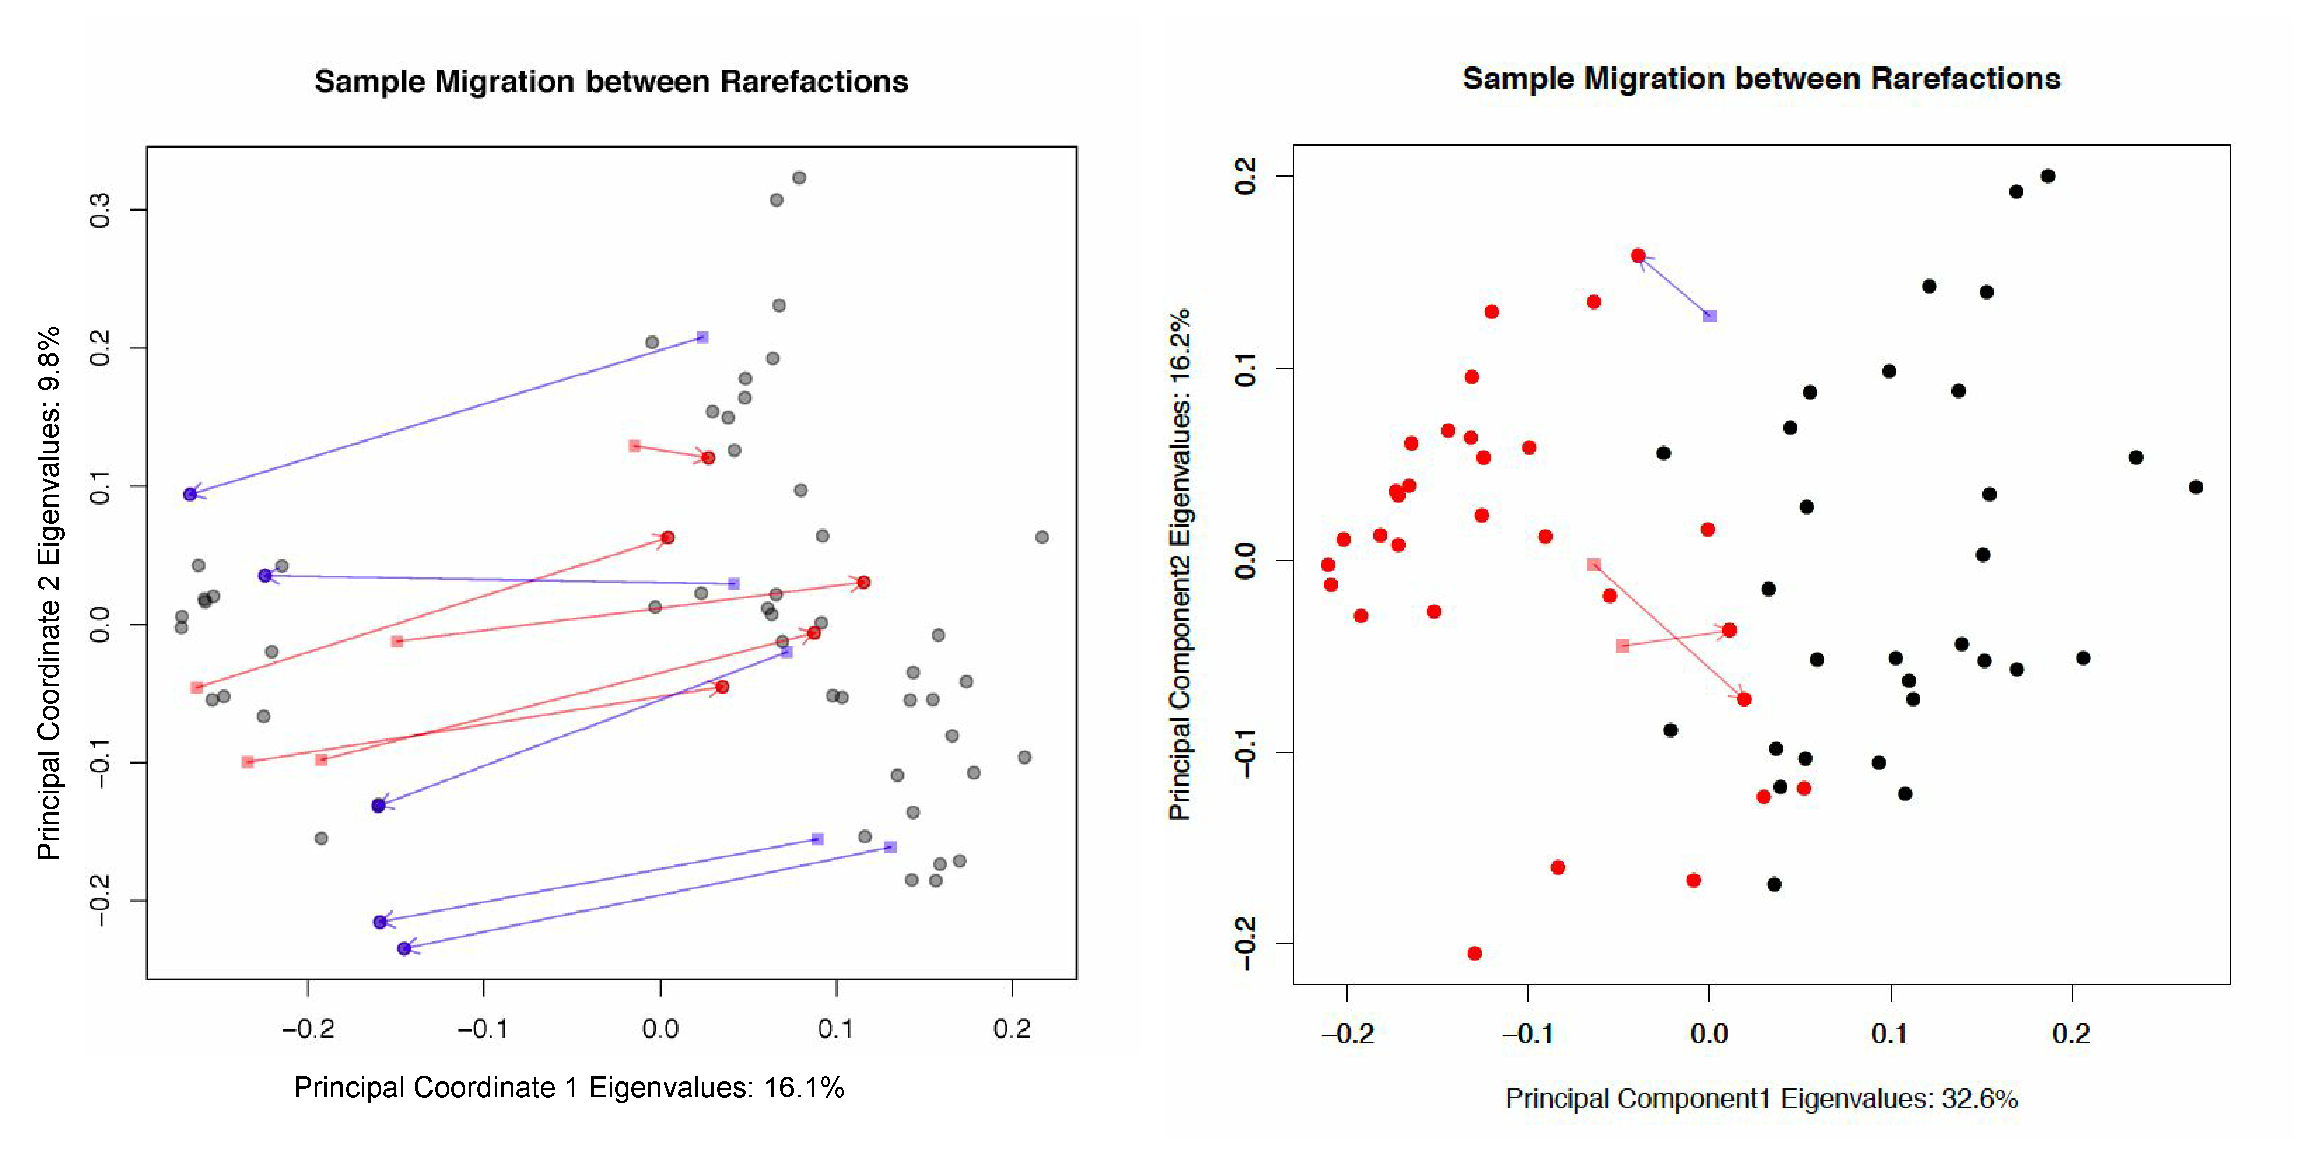
\includegraphics[scale=0.7]{/Users/dphamnyghonca/Desktop/gloor/msc_thesis_2016/unifrac_paper/sample_migration.eps}
\caption{{\bf Sample migration in different rarefactions, plotted on principal coordinates, measured with unweighted UniFrac.}
Red samples have moved from the left cluster to the right cluster between rarefactions. Blue samples have moved from the right cluster to the left. Samples are taken from the tongue dorsum body site from the Human Microbiome Project database.}
\label{fig2}
\end{figure}

Sixty tongue dorsum subsamples were drawn from the Human Microbiome Project data without replacement and filtered such that each gene had a minimum sum of 100 counts across samples. The minimum sample count for the subset of 60 we analyzed was 659, therefore we rarefied (subsampled) to the minimum of 659 to normalize the samples. For Fig.~\ref{fig2}, two independent rarefactions of the data were conducted in order to observe the effect of rarefaction variants on the metrics. The unweighted UniFrac distance was then computed for each rarefaction, and Procrustes adjustment was applied in order to overlay the second rarefaction onto the first. A PCA of rarefaction 1 was plotted, and any samples that changed between rarefactions one and two were visualized with red and blue on the plot. If the sample moved from one cluster to another between the rarefactions, it was indicated with either a blue or a red arrow. 

In both rarefactions on Fig.~\ref{fig2}, samples separated distinctly into two clusters on principal coordinate 1. Principal coordinate 1 explains the most variation in the data, and is thus useful to visualize if any associated metadata is behind the sample separation. However, the separation was not explainable by any metadata associated with the HMP experiment, and is thus an undesirable result. When plotting the rarefactions against each other, various samples are observed moving between the various clusters. This example demonstrates that samples with little difference can appear to be different through the unweighted UniFrac distance metric.

\begin{figure}[h]
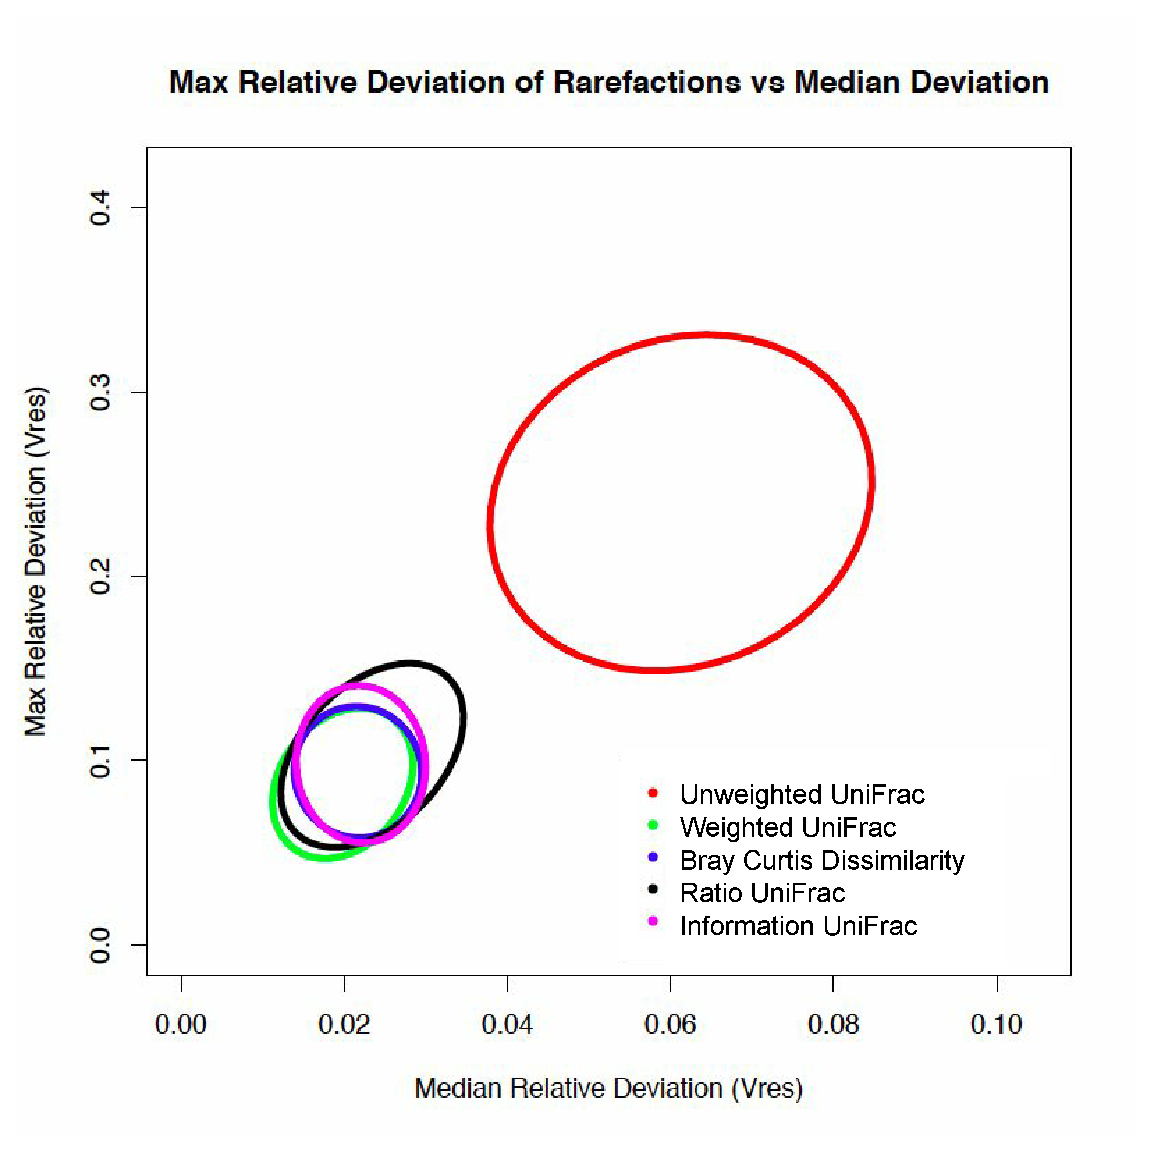
\includegraphics[scale=0.7]{/Users/dphamnyghonca/Desktop/gloor/msc_thesis_2016/unifrac_paper/ellipses.eps}
\caption{{\bf Maxiumum relative deviation of rarefactions versus median deviation for traditional and non-traditional microbiome dissimilarity metrics.} Sixty samples from the tongue dorsum were taken from the Human Microbiome Project \cite{turnbaugh2007human}, and rarefied 100 times. The maximum relative deviation was plotted against the median relative deviation of the rarefied data, and ellipses were drawn at the 95\% confidence interval, around the cloud of points for each metric. Both the maximum relative deviation of rarefied data and the median relative deviation of rarefied data are greater in unweighted UniFrac than in weighted UniFrac, Bray Curtis distance, centered ratio UniFrac, and information UniFrac.}
\label{fig3}
\end{figure}

For the ellipse plot in Fig.~\ref{fig3}, 60 tongue dorsum subsamples were randomly drawn without replacement and the gene compositions per sample were also filtered to a minimum of 100. A hundred separate rarefactions were conducted on the data to a minimum sampling depth of 378. For each individual rarefied OTU table, a distance matrix was computed using the unweighted Unifrac, weighted UniFrac, Bray-Curtis Dissimilarity, information UniFrac, and centered ratio UniFrac as a weighting method. By generating 100 separate datasets for each metric, it is possible to assess the magnitude of difference each metric has by analyzing what is essentially the same data. In other words, what does the effect of random sampling (rarefaction) have on the output of each metric? Each distance matrix generated per metric was adjusted with a Procrustes adjustment to overlay the subsequent rarefactions onto the first.

Thus, given the wide use of unweighted UniFrac in the literature with small principal component 1 and 2 effects, we suggest caution in their interpretation. For example, see the use of unweighted UniFrac in these papers about the human microbiome published in Cell\cite{hsiao2013microbiota} and Nature \cite{sonnenburg2016diet}.

The maximum value of Vres for each rarefaction is plotted against the median value per rarefaction in Fig.~\ref{fig3}. This plotting serves to highlight the maximum potential change for an analysis given that there is no difference in the data. Unweighted UniFrac shows by far the highest maximum potential change between rarefactions, compared to weighted, information, and centered ratio UniFrac, as well as Bray-Curtis.

\subsection{Why does Unweighted Unifrac have discrepancies when analyzing rarefied data?}
The UniFrac distance is defined as the sum of unshared branches divided by the sum of all branch lengths \cite{lozupone2005unifrac}. Samples that are dissimilar will have values closer to 1 as they should have more unshared branches relative to one another. Similar samples have a value closer to 0 since they will have fewer unshared branches. As defined previously, rarefaction serves the purpose of standardizing sample counts to a common denominator, which is usually defined as the lowest sequencing depth(cite rarefaction paper here). One point to note is that rarefaction carries the assumption that microbiota within samples are homogeneous and randomly distributed. However, this assumption is only valid if proper sampling protocols are observed \cite{gorzelak2015methods}. A combination of unevenly sampled genes and distantly related genes will contribute to UniFrac's variability when genes are ultimately rarefied. Distance matrices between samples will be affected when rare genes are left out during the rarefaction processes. It becomes intuitive to see how similar samples may grow dissimilar from each other through unweighted UniFrac on rarefied samples as the number of unshared branches increases as genes disappear.

\begin{figure}[h]
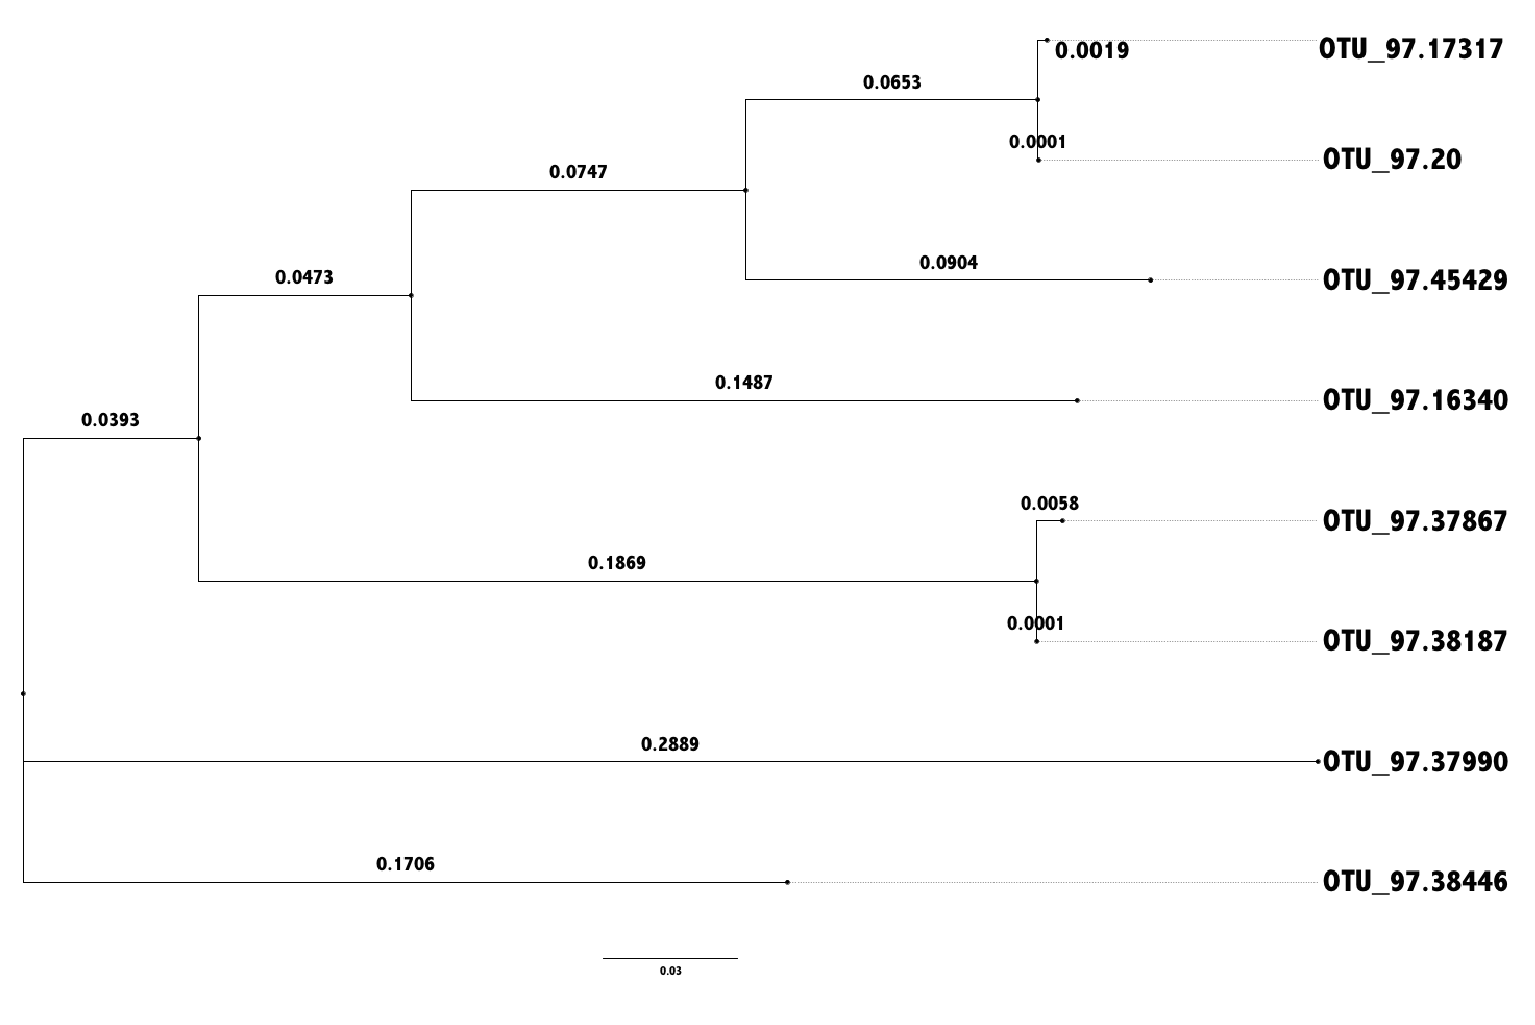
\includegraphics[scale=0.5]{/Users/dphamnyghonca/Desktop/gloor/msc_thesis_2016/unifrac_paper/tree.eps}
\caption{{\bf Phylogenetic tree with long isolated branches.}
Variation in different rarefactions of data in unweighted UniFrac analysis is exacerbated by the presence of long isolated branches in the phylogenetic tree. }
\label{fig4}
\end{figure}

\textsc{\begin{table}[!ht]
% \begin{adjustwidth}{-2.25in}{0in} % Comment out/remove adjustwidth environment if table fits in text column.
\caption{
{\bf Original abundance of taxa and rarefied abundance of taxa.} This data was simulated to demonstrate how rarefaction can change the distances reported by the unweighted UniFrac metric.}
\begin{tabular}{|l|l|l|l|l|l|l|l|}
\hline
\bf{OTU.ID} & \bf{A} & \bf{B} & \bf{\shortstack{A\\R1}} & \bf{\shortstack{B\\R1}} & \bf{\shortstack{A\\R2}} & \bf{\shortstack{B\\R2}}\\ \hline
OTU.16340 & 52 & 1 & 8 & 1 & 12 & 1\\ \hline
OTU.17317 & 17 & 4 & 3 & 4 & 5 & 4\\ \hline
OTU.20 & 70 & 18 & 14 & 18 & 20 & 18\\ \hline
OTU.37867 & 59 & 10 & 9 & 10 & 11 & 10\\ \hline
OTU.37990 & 7 & 59 & 0 & 59 & 1 & 59\\ \hline
OTU.38187 & 646 & 115 & 132 & 115 & 122 & 115\\ \hline
OTU.38446 & 6 & 8 & 0 & 8 & 1 & 8\\ \hline
OTU.45429 & 218 & 6 & 55 & 6 & 49 & 6\\ \hline
\end{tabular}
\begin{flushleft}
\end{flushleft}
\label{table1}
% \end{adjustwidth}
\end{table}}

\begin{align*}
Distance_{A:B} for Rarefaction 1 &\\
Distance_{A:B} &=\frac{\sum Unshared Branches}{\sum Total Branches}\\
&= \frac{\text{(0.2889 + 0.1706)}}{\text{1.12}}\\ 
&= \frac{\text{0.5281}}{\text{1.12}}\\ 
&= \text{0.4175}
\end{align*}

\begin{align*}
Distance_{A:B} for Rarefaction 2 &\\
Distance_{A:B} &=\frac{\sum Unshared Branches}{\sum Total Branches}\\
&= \frac{\text{0}}{\text{1.12}}\\ 
&= \text{0}
\end{align*}

With rare genes and long branch lengths in the phylogenetic tree (Fig.~\ref{fig4}), the Unweighted UniFrac distance metric on rarefied data is highly variable, declaring the samples A and B identical (distance of 0) with 1 rarefaction, and different with another (distance of 0.4175), as demonstrated in Table ~\ref{table1} and the calculations above.

While an improvement on unweighted UniFrac, weighted UniFrac can overweight differences between large proportional abundances and underweight differences between small proportional abundances. If one bacterial taxa increased in proportion from 5/1000 to 10/1000 and another taxa increased in proportion from 95/1000 to 100/1000, they would have the same weight in weighted UniFrac. However, the first taxa has doubled in proportion between samples, and this is much more biologically significant than the change in proportional abundance in the second taxa. Additionally, it does not account for how the counts add up to a constrained sum determined by the sequencing machine model. Because the sum is constrained, as an example, an increase in growth of one taxa can make the data look like there is a decrease in abundance in other taxa, even if in reality the population of the other taxa stayed the same.

Here we explore some alternatives to unweighted and weighted UniFrac, and discuss their merits and shortfalls.

\subsection{Information UniFrac}

The difference in information content between low proportional abundances (which make up the bulk of microbiome data) is generally higher than the difference between the proportional abundances themselves, potentially allowing scientists to differentiate groups with subtle differences.

\begin{figure}[h]
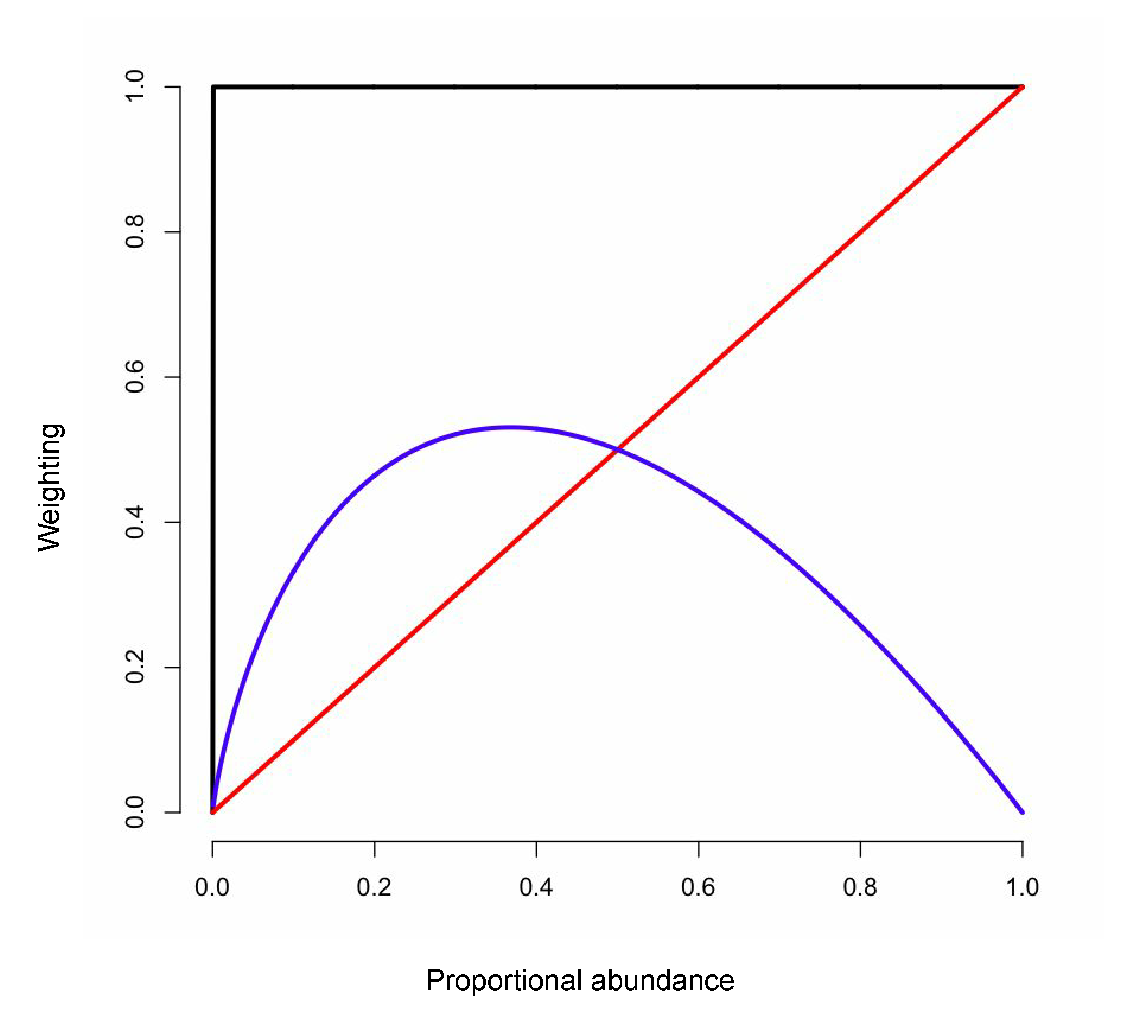
\includegraphics[scale=0.6]{/Users/dphamnyghonca/Desktop/gloor/msc_thesis_2016/unifrac_paper/weightings.eps}
\caption{{\bf Unifrac weights. }
Each UniFrac weighting is plotted with the corresponding proportional abundance. The black line is unweighted UniFrac, the red line is weighted UniFrac,and  the blue line is information UniFrac. }
\label{fig5}
\end{figure}

Near the 0, 0 point in Fig.~\ref{fig5}, the proportional abundances are low. Here there is higher differentiation between weights of different pairs of low proportional abundances for information UniFrac, as shown by the higher slope of the curved graph. The centered ratio UniFrac (not depicted) depends on the geometric mean of the taxonomic abundances, and would have a different slope in the weight graph depending on how evenly the abundances were distributed.

\subsection{Tongue and cheek comparison}

\begin{figure}[h]
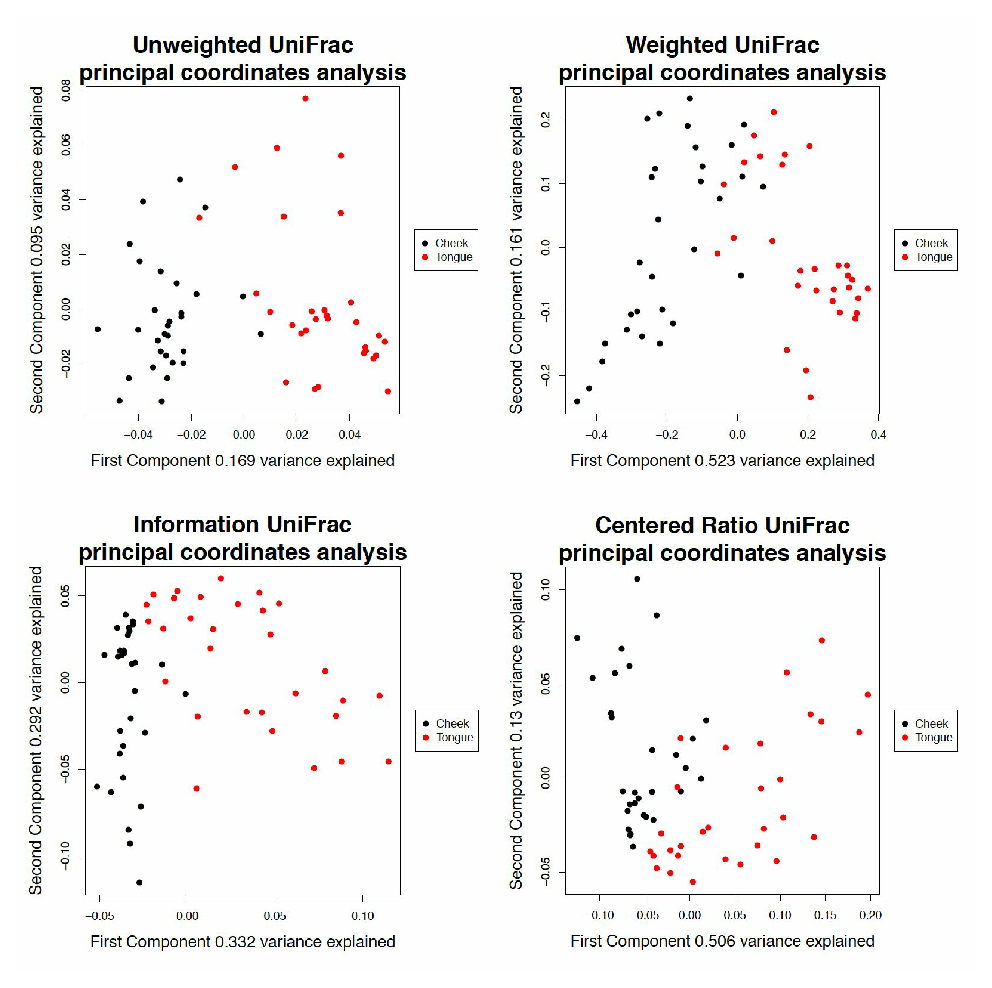
\includegraphics[scale=0.8]{/Users/dphamnyghonca/Desktop/gloor/msc_thesis_2016/unifrac_paper/tongue_cheek.eps}
\caption{{\bf Analysis of tongue and cheek data using different UniFrac weightings. }
A principal coordinate analysis of a 16S rRNA experiment done on samples from the tongue and cheek, selected from the Human Microbiome Project \cite{turnbaugh2007human}. All weightings show separation between the samples by body site. }
\label{fig6}
\end{figure}

We next explore two other datasets, one with a defined difference between groups (tongue dorsum compared to buccal mucosa), and one with an outlier that is only apparent when analyzed by certain dissimilarity metrics.

Fig.~\ref{fig6} shows a principal coordinate analysis plot with four different metrics: unweighted UniFrac, weighted UniFrac, information UniFrac, and centered ratio UniFrac. We observe that the difference in the microbiome between the human tongue and cheek are well defined by all metrics (Fig.~\ref{fig6}), since all of the weightings show separation between the samples according to body site. We conclude that weighted UniFrac, information UniFrac, and centered ratio UniFrac do not tend to show spurious separation in uniform data sets to the degree that unweighted UniFrac does (Fig.~\ref{fig3}), while reliably separating samples in data with a defined difference between groups.

\subsection{Breast milk Data}

\begin{figure}[h]
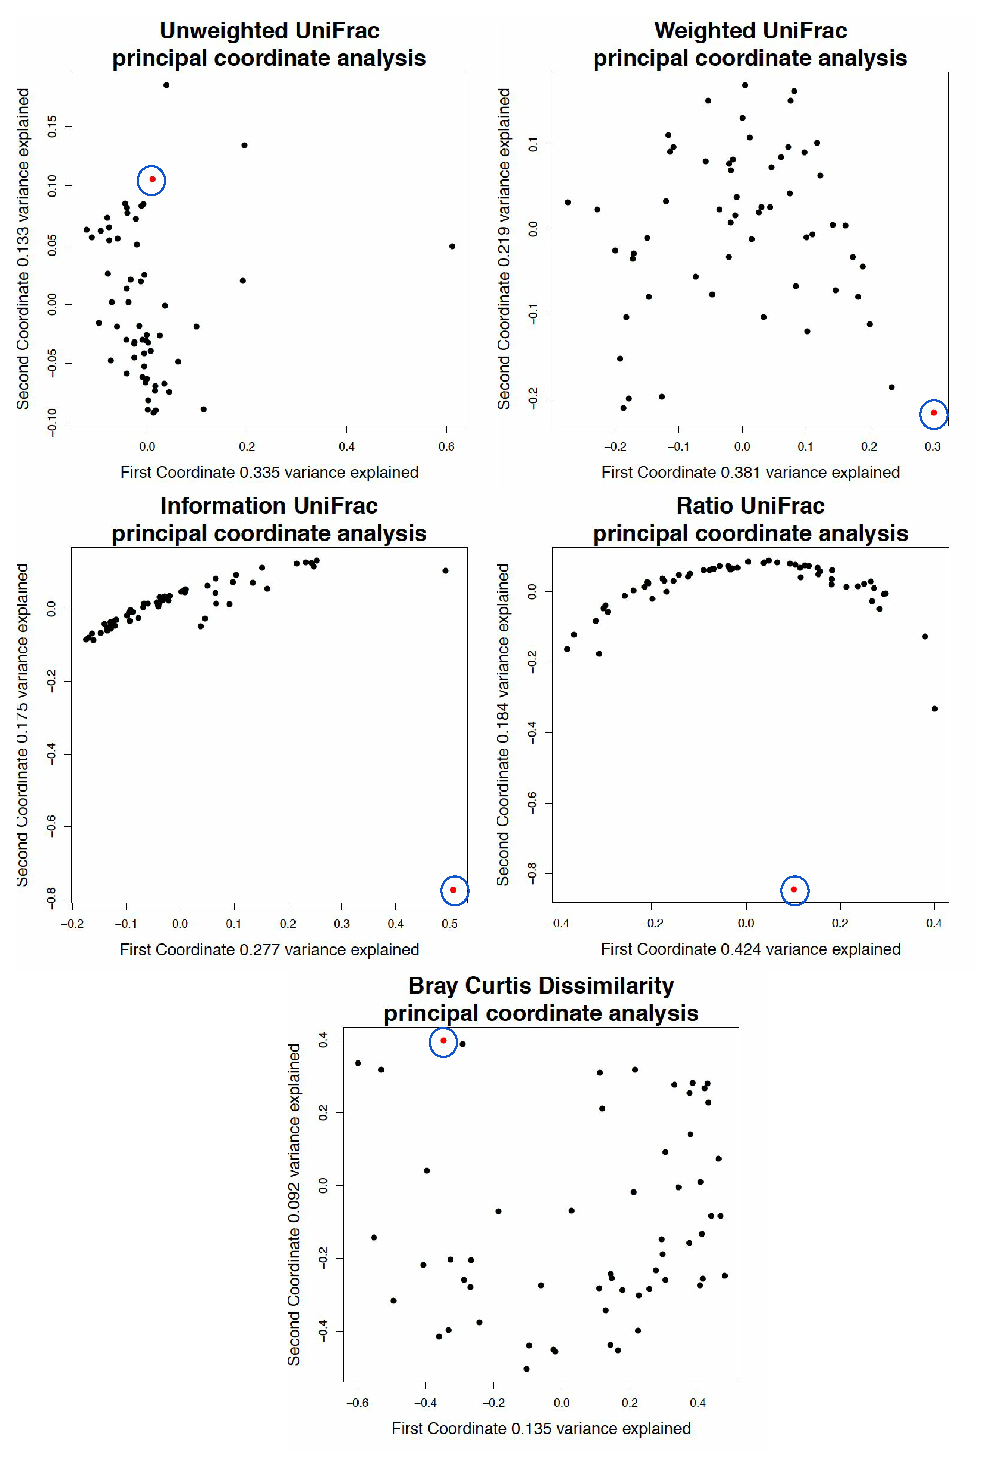
\includegraphics[scale=0.8]{/Users/dphamnyghonca/Desktop/gloor/msc_thesis_2016/unifrac_paper/breastmilk.eps}
\caption{{\bf Analysis of breast milk data using different UniFrac weightings. }
A principal coordinate analysis of a 16S rRNA experiment done on samples from a 16S rRNA experiment on breast milk. The circled sample is infected with 97\% \textit{Pseudomonas}, compared to 15-20\% in the other samples. }
\label{fig7}
\end{figure}

Fig.~\ref{fig7} is a principal coordinate analysis of a 16S rRNA gene sequencing experiment done on microbiome samples from breast milk \cite{urbaniak2016human}. Breast milk samples were collected and the V4 region of the 16S rRNA gene was sequenced. One of these samples was infected (circled), consisting of 97\% Pasteurella. We noted that this sample was not distinct in unweighted and weighted UniFrac because the distance from the Pasteurella branches of the phylogenetic tree to the root of the tree (rooted by midpoint) were not particularly short or long, measuring at just over the 3rd quartile of all root-to-leaf distances. In addition, the Pasteurella leaves shared a clade with many other taxa.

The reason the infected sample in the breast milk study is so distinct from the rest of the samples in Information UniFrac and Centered Ratio UniFrac is because of the weighting. The infected sample was 97\% Pasteurella, while the other samples generally had 15-20\% each of Staphylococcus and Pseudomonas, and little or no Pasteurella. Unweighted UniFrac does not differentiate between high and low abundance. Weighted UniFrac does, placing the infected sample in the bottom right corner of that plot. Information UniFrac weights everything in the infected sample close to zero, as taxa are present in either very high or very low abundance, while weighting Staphylococcus and Pseudomonas in the other samples highly (around 0.4) due to their 15-20\% abundance. Centered ratio UniFrac recognizes that the infected sample has a taxonomic abundance very far from the geometric mean abundance. For these reasons information and centered ratio UniFrac are more adept at picking up outliers with uneven distributions, even if the taxa are shared by other samples.

\section*{Discussion}
As shown in the tongue and cheek data set, unweighted UniFrac is perfectly sufficient for data sets with a notable difference. However, in data sets with no difference or a very small difference between groups such the uniform tongue dorsum data set, unweighted UniFrac is the least reliable and we found that it may produce wildly different results depending on rarefaction and sequencing depth. This can result in spurious groups, or inclusion of samples in the wrong groups.

We found weighted UniFrac, information UniFrac, centered ratio UniFrac, and Bray-Curtis methods to be more reliable choices. We suggest that investigators use several methods as they can detect outliers in different circumstances. When an outlier is detected by any metric, an investigation is warranted, as with our example in the breast milk data set.

In summary, with the addition of information UniFrac and centered ratio UniFrac, biologists have more tools at their disposal to prevent spurious interpretations, detect outliers, and ultimately understand their data better.

\section*{Acknowledgments}
Thanks to Camilla Urbaniak for providing the data from her breast milk study \cite{urbaniak2016human}.

\nolinenumbers

%\section*{References}
% Either type in your references using
% \begin{thebibliography}{}
% \bibitem{}
% Text
% \end{thebibliography}
%
% OR
%
% Compile your BiBTeX database using our plos2015.bst
% style file and paste the contents of your .bbl file
% here.
% 
\bibliography{unifrac}



\end{document}

